\documentclass[1p]{elsarticle_modified}
%\bibliographystyle{elsarticle-num}

%\usepackage[colorlinks]{hyperref}
%\usepackage{abbrmath_seonhwa} %\Abb, \Ascr, \Acal ,\Abf, \Afrak
\usepackage{amsfonts}
\usepackage{amssymb}
\usepackage{amsmath}
\usepackage{amsthm}
\usepackage{scalefnt}
\usepackage{amsbsy}
\usepackage{kotex}
\usepackage{caption}
\usepackage{subfig}
\usepackage{color}
\usepackage{graphicx}
\usepackage{xcolor} %% white, black, red, green, blue, cyan, magenta, yellow
\usepackage{float}
\usepackage{setspace}
\usepackage{hyperref}

\usepackage{tikz}
\usetikzlibrary{arrows}

\usepackage{multirow}
\usepackage{array} % fixed length table
\usepackage{hhline}

%%%%%%%%%%%%%%%%%%%%%
\makeatletter
\renewcommand*\env@matrix[1][\arraystretch]{%
	\edef\arraystretch{#1}%
	\hskip -\arraycolsep
	\let\@ifnextchar\new@ifnextchar
	\array{*\c@MaxMatrixCols c}}
\makeatother %https://tex.stackexchange.com/questions/14071/how-can-i-increase-the-line-spacing-in-a-matrix
%%%%%%%%%%%%%%%

\usepackage[normalem]{ulem}

\newcommand{\msout}[1]{\ifmmode\text{\sout{\ensuremath{#1}}}\else\sout{#1}\fi}
%SOURCE: \msout is \stkout macro in https://tex.stackexchange.com/questions/20609/strikeout-in-math-mode

\newcommand{\cancel}[1]{
	\ifmmode
	{\color{red}\msout{#1}}
	\else
	{\color{red}\sout{#1}}
	\fi
}

\newcommand{\add}[1]{
	{\color{blue}\uwave{#1}}
}

\newcommand{\replace}[2]{
	\ifmmode
	{\color{red}\msout{#1}}{\color{blue}\uwave{#2}}
	\else
	{\color{red}\sout{#1}}{\color{blue}\uwave{#2}}
	\fi
}

\newcommand{\Sol}{\mathcal{S}} %segment
\newcommand{\D}{D} %diagram
\newcommand{\A}{\mathcal{A}} %arc


%%%%%%%%%%%%%%%%%%%%%%%%%%%%%5 test

\def\sl{\operatorname{\textup{SL}}(2,\Cbb)}
\def\psl{\operatorname{\textup{PSL}}(2,\Cbb)}
\def\quan{\mkern 1mu \triangleright \mkern 1mu}

\theoremstyle{definition}
\newtheorem{thm}{Theorem}[section]
\newtheorem{prop}[thm]{Proposition}
\newtheorem{lem}[thm]{Lemma}
\newtheorem{ques}[thm]{Question}
\newtheorem{cor}[thm]{Corollary}
\newtheorem{defn}[thm]{Definition}
\newtheorem{exam}[thm]{Example}
\newtheorem{rmk}[thm]{Remark}
\newtheorem{alg}[thm]{Algorithm}

\newcommand{\I}{\sqrt{-1}}
\begin{document}

%\begin{frontmatter}
%
%\title{Boundary parabolic representations of knots up to 8 crossings}
%
%%% Group authors per affiliation:
%\author{Yunhi Cho} 
%\address{Department of Mathematics, University of Seoul, Seoul, Korea}
%\ead{yhcho@uos.ac.kr}
%
%
%\author{Seonhwa Kim} %\fnref{s_kim}}
%\address{Center for Geometry and Physics, Institute for Basic Science, Pohang, 37673, Korea}
%\ead{ryeona17@ibs.re.kr}
%
%\author{Hyuk Kim}
%\address{Department of Mathematical Sciences, Seoul National University, Seoul 08826, Korea}
%\ead{hyukkim@snu.ac.kr}
%
%\author{Seokbeom Yoon}
%\address{Department of Mathematical Sciences, Seoul National University, Seoul, 08826,  Korea}
%\ead{sbyoon15@snu.ac.kr}
%
%\begin{abstract}
%We find all boundary parabolic representation of knots up to 8 crossings.
%
%\end{abstract}
%\begin{keyword}
%    \MSC[2010] 57M25 
%\end{keyword}
%
%\end{frontmatter}

%\linenumbers
%\tableofcontents
%
\newcommand\colored[1]{\textcolor{white}{\rule[-0.35ex]{0.8em}{1.4ex}}\kern-0.8em\color{red} #1}%
%\newcommand\colored[1]{\textcolor{white}{ #1}\kern-2.17ex	\textcolor{white}{ #1}\kern-1.81ex	\textcolor{white}{ #1}\kern-2.15ex\color{red}#1	}

{\Large $\underline{12a_{0628}~(K12a_{0628})}$}

\setlength{\tabcolsep}{10pt}
\renewcommand{\arraystretch}{1.6}
\vspace{1cm}\begin{tabular}{m{100pt}>{\centering\arraybackslash}m{274pt}}
\multirow{5}{120pt}{
	\centering
	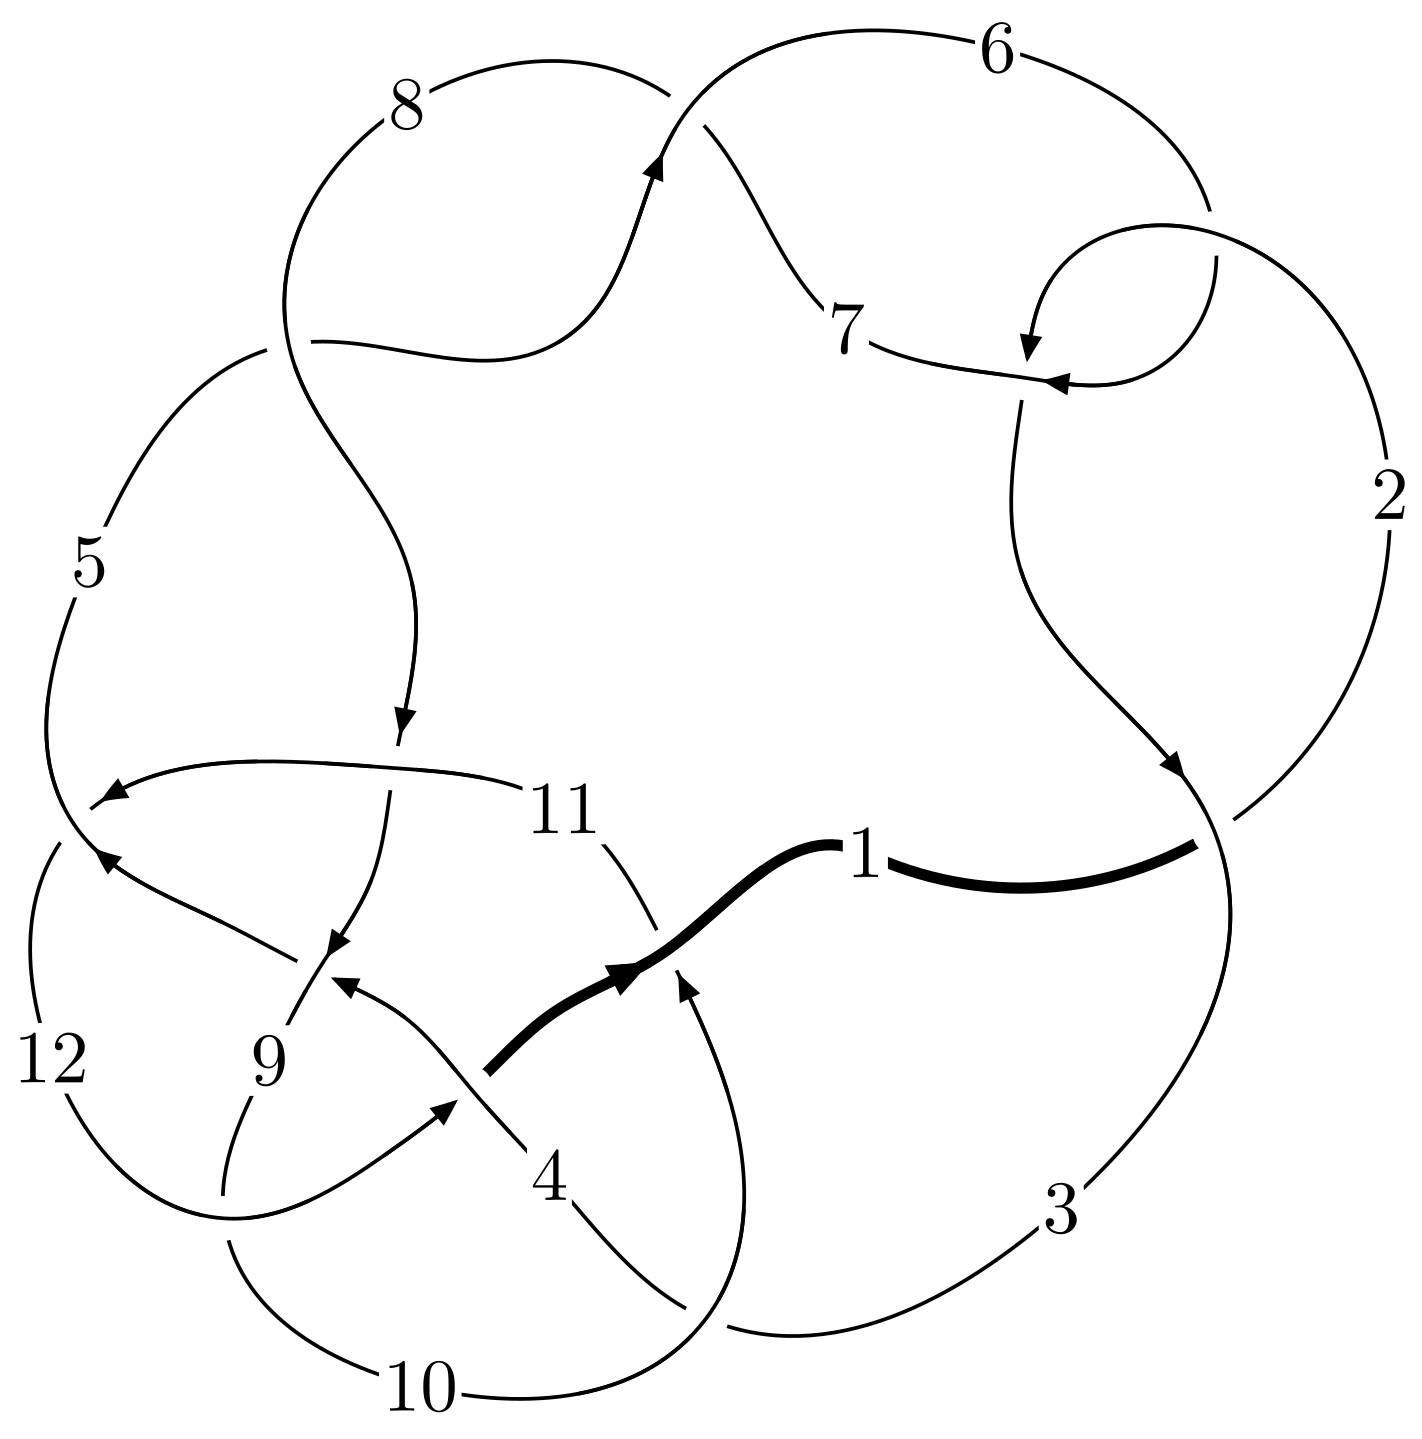
\includegraphics[width=112pt]{../../../GIT/diagram.site/Diagrams/png/1429_12a_0628.png}\\
\ \ \ A knot diagram\footnotemark}&
\allowdisplaybreaks
\textbf{Linearized knot diagam} \\
\cline{2-2}
 &
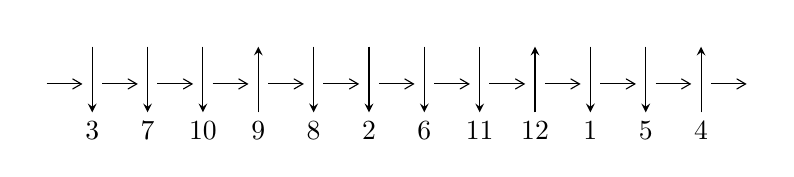
\begin{tikzpicture}[x=20pt, y=17pt]
	% nodes
	\node (C0) at (0, 0) {};
	\node (C1) at (1, 0) {};
	\node (C1U) at (1, +1) {};
	\node (C1D) at (1, -1) {3};

	\node (C2) at (2, 0) {};
	\node (C2U) at (2, +1) {};
	\node (C2D) at (2, -1) {7};

	\node (C3) at (3, 0) {};
	\node (C3U) at (3, +1) {};
	\node (C3D) at (3, -1) {10};

	\node (C4) at (4, 0) {};
	\node (C4U) at (4, +1) {};
	\node (C4D) at (4, -1) {9};

	\node (C5) at (5, 0) {};
	\node (C5U) at (5, +1) {};
	\node (C5D) at (5, -1) {8};

	\node (C6) at (6, 0) {};
	\node (C6U) at (6, +1) {};
	\node (C6D) at (6, -1) {2};

	\node (C7) at (7, 0) {};
	\node (C7U) at (7, +1) {};
	\node (C7D) at (7, -1) {6};

	\node (C8) at (8, 0) {};
	\node (C8U) at (8, +1) {};
	\node (C8D) at (8, -1) {11};

	\node (C9) at (9, 0) {};
	\node (C9U) at (9, +1) {};
	\node (C9D) at (9, -1) {12};

	\node (C10) at (10, 0) {};
	\node (C10U) at (10, +1) {};
	\node (C10D) at (10, -1) {1};

	\node (C11) at (11, 0) {};
	\node (C11U) at (11, +1) {};
	\node (C11D) at (11, -1) {5};

	\node (C12) at (12, 0) {};
	\node (C12U) at (12, +1) {};
	\node (C12D) at (12, -1) {4};
	\node (C13) at (13, 0) {};

	% arrows
	\draw[->,>={angle 60}]
	(C0) edge (C1) (C1) edge (C2) (C2) edge (C3) (C3) edge (C4) (C4) edge (C5) (C5) edge (C6) (C6) edge (C7) (C7) edge (C8) (C8) edge (C9) (C9) edge (C10) (C10) edge (C11) (C11) edge (C12) (C12) edge (C13) ;	\draw[->,>=stealth]
	(C1U) edge (C1D) (C2U) edge (C2D) (C3U) edge (C3D) (C4D) edge (C4U) (C5U) edge (C5D) (C6U) edge (C6D) (C7U) edge (C7D) (C8U) edge (C8D) (C9D) edge (C9U) (C10U) edge (C10D) (C11U) edge (C11D) (C12D) edge (C12U) ;
	\end{tikzpicture} \\
\hhline{~~} \\& 
\textbf{Solving Sequence} \\ \cline{2-2} 
 &
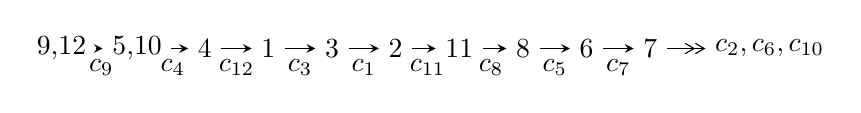
\begin{tikzpicture}[x=23pt, y=7pt]
	% node
	\node (A0) at (-1/8, 0) {9,12};
	\node (A1) at (17/16, 0) {5,10};
	\node (A2) at (17/8, 0) {4};
	\node (A3) at (25/8, 0) {1};
	\node (A4) at (33/8, 0) {3};
	\node (A5) at (41/8, 0) {2};
	\node (A6) at (49/8, 0) {11};
	\node (A7) at (57/8, 0) {8};
	\node (A8) at (65/8, 0) {6};
	\node (A9) at (73/8, 0) {7};
	\node (C1) at (1/2, -1) {$c_{9}$};
	\node (C2) at (13/8, -1) {$c_{4}$};
	\node (C3) at (21/8, -1) {$c_{12}$};
	\node (C4) at (29/8, -1) {$c_{3}$};
	\node (C5) at (37/8, -1) {$c_{1}$};
	\node (C6) at (45/8, -1) {$c_{11}$};
	\node (C7) at (53/8, -1) {$c_{8}$};
	\node (C8) at (61/8, -1) {$c_{5}$};
	\node (C9) at (69/8, -1) {$c_{7}$};
	\node (A10) at (11, 0) {$c_{2},c_{6},c_{10}$};

	% edge
	\draw[->,>=stealth]	
	(A0) edge (A1) (A1) edge (A2) (A2) edge (A3) (A3) edge (A4) (A4) edge (A5) (A5) edge (A6) (A6) edge (A7) (A7) edge (A8) (A8) edge (A9) ;
	\draw[->>,>={angle 60}]	
	(A9) edge (A10);
\end{tikzpicture} \\ 

\end{tabular} \\

\footnotetext{
The image of knot diagram is generated by the software ``\textbf{Draw programme}" developed by Andrew Bartholomew(\url{http://www.layer8.co.uk/maths/draw/index.htm\#Running-draw}), where we modified some parts for our purpose(\url{https://github.com/CATsTAILs/LinksPainter}).
}\phantom \\ \newline 
\centering \textbf{Ideals for irreducible components\footnotemark of $X_{\text{par}}$} 
 
\begin{align*}
I^u_{1}&=\langle 
-8.07461\times10^{68} u^{46}+1.87630\times10^{70} u^{45}+\cdots+3.58440\times10^{69} b+2.42033\times10^{69},\\
\phantom{I^u_{1}}&\phantom{= \langle  }-4.03525\times10^{69} u^{46}+9.96490\times10^{70} u^{45}+\cdots+7.16879\times10^{69} a-2.41381\times10^{70},\\
\phantom{I^u_{1}}&\phantom{= \langle  }u^{47}-25 u^{46}+\cdots+9 u-2\rangle \\
I^u_{2}&=\langle 
2 u^{34} a+9 u^{34}+\cdots-16 a-66,\;74 u^{34} a+11 u^{34}+\cdots-1408 a-380,\;u^{35}+17 u^{34}+\cdots-36 u-8\rangle \\
I^u_{3}&=\langle 
- u^{13}-11 u^{12}+\cdots+b-69,\;-50 u^{13}-600 u^{12}+\cdots+119 a-5520,\;u^{14}+12 u^{13}+\cdots+753 u+119\rangle \\
\\
I^v_{1}&=\langle 
a,\;6 v^5-52 v^4+157 v^3-196 v^2+b+114 v-20,\;v^6-9 v^5+29 v^4-41 v^3+29 v^2-9 v+1\rangle \\
\end{align*}
\raggedright * 4 irreducible components of $\dim_{\mathbb{C}}=0$, with total 137 representations.\\
\footnotetext{All coefficients of polynomials are rational numbers. But the coefficients are sometimes approximated in decimal forms when there is not enough margin.}
\newpage
\renewcommand{\arraystretch}{1}
\centering \section*{I. $I^u_{1}= \langle -8.07\times10^{68} u^{46}+1.88\times10^{70} u^{45}+\cdots+3.58\times10^{69} b+2.42\times10^{69},\;-4.04\times10^{69} u^{46}+9.96\times10^{70} u^{45}+\cdots+7.17\times10^{69} a-2.41\times10^{70},\;u^{47}-25 u^{46}+\cdots+9 u-2 \rangle$}
\flushleft \textbf{(i) Arc colorings}\\
\begin{tabular}{m{7pt} m{180pt} m{7pt} m{180pt} }
\flushright $a_{9}=$&$\begin{pmatrix}1\\0\end{pmatrix}$ \\
\flushright $a_{12}=$&$\begin{pmatrix}0\\u\end{pmatrix}$ \\
\flushright $a_{5}=$&$\begin{pmatrix}0.562891 u^{46}-13.9004 u^{45}+\cdots-5.16569 u+3.36710\\0.225271 u^{46}-5.23462 u^{45}+\cdots-1.00376 u-0.675240\end{pmatrix}$ \\
\flushright $a_{10}=$&$\begin{pmatrix}1\\- u^2\end{pmatrix}$ \\
\flushright $a_{4}=$&$\begin{pmatrix}0.337620 u^{46}-8.66577 u^{45}+\cdots-4.16193 u+4.04234\\0.225271 u^{46}-5.23462 u^{45}+\cdots-1.00376 u-0.675240\end{pmatrix}$ \\
\flushright $a_{1}=$&$\begin{pmatrix}0.169203 u^{46}-4.28920 u^{45}+\cdots-7.93593 u+2.72071\\0.0591214 u^{46}-1.09993 u^{45}+\cdots-0.197882 u-0.338406\end{pmatrix}$ \\
\flushright $a_{3}=$&$\begin{pmatrix}0.165732 u^{46}-4.51075 u^{45}+\cdots-2.46301 u+2.91656\\0.435105 u^{46}-10.3002 u^{45}+\cdots-1.93948 u-0.390908\end{pmatrix}$ \\
\flushright $a_{2}=$&$\begin{pmatrix}0.0648503 u^{46}-1.39194 u^{45}+\cdots-14.5959 u+2.04861\\-0.131505 u^{46}+3.30763 u^{45}+\cdots-0.786389 u+0.0263510\end{pmatrix}$ \\
\flushright $a_{11}=$&$\begin{pmatrix}-0.0906579 u^{46}+2.39136 u^{45}+\cdots-9.46119 u+1.92565\\-0.318982 u^{46}+7.78049 u^{45}+\cdots+0.672616 u-0.456649\end{pmatrix}$ \\
\flushright $a_{8}=$&$\begin{pmatrix}0.242494 u^{46}-6.10090 u^{45}+\cdots+14.2499 u-0.538109\\0.220995 u^{46}-5.44044 u^{45}+\cdots+0.632902 u+0.206826\end{pmatrix}$ \\
\flushright $a_{6}=$&$\begin{pmatrix}0.593189 u^{46}-14.8971 u^{45}+\cdots+5.69357 u+1.97676\\0.561061 u^{46}-13.2944 u^{45}+\cdots-0.319039 u-0.574337\end{pmatrix}$ \\
\flushright $a_{7}=$&$\begin{pmatrix}0.784381 u^{46}-19.6156 u^{45}+\cdots+14.2320 u+1.32228\\0.322833 u^{46}-7.50881 u^{45}+\cdots+2.82860 u-0.790986\end{pmatrix}$\\&\end{tabular}
\flushleft \textbf{(ii) Obstruction class $= -1$}\\~\\
\flushleft \textbf{(iii) Cusp Shapes $= 0.442403 u^{46}-9.99419 u^{45}+\cdots-2.55500 u-6.13236$}\\~\\
\newpage\renewcommand{\arraystretch}{1}
\flushleft \textbf{(iv) u-Polynomials at the component}\newline \\
\begin{tabular}{m{50pt}|m{274pt}}
Crossings & \hspace{64pt}u-Polynomials at each crossing \\
\hline $$\begin{aligned}c_{1},c_{5},c_{7}\end{aligned}$$&$\begin{aligned}
&u^{47}+11 u^{46}+\cdots+129 u+16
\end{aligned}$\\
\hline $$\begin{aligned}c_{2},c_{6}\end{aligned}$$&$\begin{aligned}
&u^{47}-5 u^{46}+\cdots+5 u+4
\end{aligned}$\\
\hline $$\begin{aligned}c_{3},c_{11}\end{aligned}$$&$\begin{aligned}
&u^{47}+9 u^{45}+\cdots-6 u+1
\end{aligned}$\\
\hline $$\begin{aligned}c_{4},c_{12}\end{aligned}$$&$\begin{aligned}
&u^{47}+3 u^{46}+\cdots+3 u+1
\end{aligned}$\\
\hline $$\begin{aligned}c_{8},c_{10}\end{aligned}$$&$\begin{aligned}
&u^{47}+8 u^{46}+\cdots+14 u-1
\end{aligned}$\\
\hline $$\begin{aligned}c_{9}\end{aligned}$$&$\begin{aligned}
&u^{47}+25 u^{46}+\cdots+9 u+2
\end{aligned}$\\
\hline
\end{tabular}\\~\\
\newpage\renewcommand{\arraystretch}{1}
\flushleft \textbf{(v) Riley Polynomials at the component}\newline \\
\begin{tabular}{m{50pt}|m{274pt}}
Crossings & \hspace{64pt}Riley Polynomials at each crossing \\
\hline $$\begin{aligned}c_{1},c_{5},c_{7}\end{aligned}$$&$\begin{aligned}
&y^{47}+53 y^{46}+\cdots-12319 y-256
\end{aligned}$\\
\hline $$\begin{aligned}c_{2},c_{6}\end{aligned}$$&$\begin{aligned}
&y^{47}-11 y^{46}+\cdots+129 y-16
\end{aligned}$\\
\hline $$\begin{aligned}c_{3},c_{11}\end{aligned}$$&$\begin{aligned}
&y^{47}+18 y^{46}+\cdots+24 y-1
\end{aligned}$\\
\hline $$\begin{aligned}c_{4},c_{12}\end{aligned}$$&$\begin{aligned}
&y^{47}+29 y^{46}+\cdots-53 y-1
\end{aligned}$\\
\hline $$\begin{aligned}c_{8},c_{10}\end{aligned}$$&$\begin{aligned}
&y^{47}-6 y^{46}+\cdots+316 y-1
\end{aligned}$\\
\hline $$\begin{aligned}c_{9}\end{aligned}$$&$\begin{aligned}
&y^{47}-3 y^{46}+\cdots+109 y-4
\end{aligned}$\\
\hline
\end{tabular}\\~\\
\newpage\flushleft \textbf{(vi) Complex Volumes and Cusp Shapes}
$$\begin{array}{c|c|c}  
\text{Solutions to }I^u_{1}& \I (\text{vol} + \sqrt{-1}CS) & \text{Cusp shape}\\
 \hline 
\begin{aligned}
u &= \phantom{-}0.986892 + 0.257612 I \\
a &= -0.240592 + 0.022595 I \\
b &= -0.105712 + 0.949661 I\end{aligned}
 & -1.56579 + 2.13171 I & \phantom{-0.000000 } 0 \\ \hline\begin{aligned}
u &= \phantom{-}0.986892 - 0.257612 I \\
a &= -0.240592 - 0.022595 I \\
b &= -0.105712 - 0.949661 I\end{aligned}
 & -1.56579 - 2.13171 I & \phantom{-0.000000 } 0 \\ \hline\begin{aligned}
u &= -0.830353 + 0.249534 I \\
a &= \phantom{-}0.156117 - 0.996332 I \\
b &= -0.000476 - 0.473342 I\end{aligned}
 & \phantom{-}1.96281 - 2.11633 I & \phantom{-0.000000 -}0. + 4.02661 I \\ \hline\begin{aligned}
u &= -0.830353 - 0.249534 I \\
a &= \phantom{-}0.156117 + 0.996332 I \\
b &= -0.000476 + 0.473342 I\end{aligned}
 & \phantom{-}1.96281 + 2.11633 I & \phantom{-0.000000 } 0. - 4.02661 I \\ \hline\begin{aligned}
u &= \phantom{-}1.045570 + 0.455359 I \\
a &= \phantom{-}0.231147 - 0.651269 I \\
b &= -1.13460 - 1.29557 I\end{aligned}
 & -1.01169 + 1.42980 I & \phantom{-0.000000 } 0 \\ \hline\begin{aligned}
u &= \phantom{-}1.045570 - 0.455359 I \\
a &= \phantom{-}0.231147 + 0.651269 I \\
b &= -1.13460 + 1.29557 I\end{aligned}
 & -1.01169 - 1.42980 I & \phantom{-0.000000 } 0 \\ \hline\begin{aligned}
u &= \phantom{-}0.779229 + 0.975300 I \\
a &= -0.537680 + 0.259174 I \\
b &= -0.166184 + 0.726379 I\end{aligned}
 & -4.20569 - 1.69908 I & \phantom{-0.000000 } 0 \\ \hline\begin{aligned}
u &= \phantom{-}0.779229 - 0.975300 I \\
a &= -0.537680 - 0.259174 I \\
b &= -0.166184 - 0.726379 I\end{aligned}
 & -4.20569 + 1.69908 I & \phantom{-0.000000 } 0 \\ \hline\begin{aligned}
u &= \phantom{-}0.183042 + 0.680484 I \\
a &= \phantom{-}0.931695 - 0.444316 I \\
b &= -0.009062 - 0.684052 I\end{aligned}
 & -0.97551 - 1.07913 I & -5.53069 + 4.56519 I \\ \hline\begin{aligned}
u &= \phantom{-}0.183042 - 0.680484 I \\
a &= \phantom{-}0.931695 + 0.444316 I \\
b &= -0.009062 + 0.684052 I\end{aligned}
 & -0.97551 + 1.07913 I & -5.53069 - 4.56519 I\\
 \hline 
 \end{array}$$\newpage$$\begin{array}{c|c|c}  
\text{Solutions to }I^u_{1}& \I (\text{vol} + \sqrt{-1}CS) & \text{Cusp shape}\\
 \hline 
\begin{aligned}
u &= \phantom{-}1.202810 + 0.603274 I \\
a &= -0.086506 + 0.756693 I \\
b &= \phantom{-}0.99713 + 1.26439 I\end{aligned}
 & \phantom{-}1.79955 + 5.97631 I & \phantom{-0.000000 } 0 \\ \hline\begin{aligned}
u &= \phantom{-}1.202810 - 0.603274 I \\
a &= -0.086506 - 0.756693 I \\
b &= \phantom{-}0.99713 - 1.26439 I\end{aligned}
 & \phantom{-}1.79955 - 5.97631 I & \phantom{-0.000000 } 0 \\ \hline\begin{aligned}
u &= \phantom{-}1.104270 + 0.787113 I \\
a &= \phantom{-}0.119630 - 0.908657 I \\
b &= -0.99509 - 1.20831 I\end{aligned}
 & -3.04962 + 8.17588 I & \phantom{-0.000000 } 0 \\ \hline\begin{aligned}
u &= \phantom{-}1.104270 - 0.787113 I \\
a &= \phantom{-}0.119630 + 0.908657 I \\
b &= -0.99509 + 1.20831 I\end{aligned}
 & -3.04962 - 8.17588 I & \phantom{-0.000000 } 0 \\ \hline\begin{aligned}
u &= \phantom{-}0.304094 + 1.336820 I \\
a &= \phantom{-}0.542187 - 0.423730 I \\
b &= \phantom{-}0.126684 - 0.613012 I\end{aligned}
 & -0.33080 - 2.07585 I & \phantom{-0.000000 } 0 \\ \hline\begin{aligned}
u &= \phantom{-}0.304094 - 1.336820 I \\
a &= \phantom{-}0.542187 + 0.423730 I \\
b &= \phantom{-}0.126684 + 0.613012 I\end{aligned}
 & -0.33080 + 2.07585 I & \phantom{-0.000000 } 0 \\ \hline\begin{aligned}
u &= \phantom{-}0.137187 + 0.560954 I \\
a &= \phantom{-}1.24351 - 1.45572 I \\
b &= -0.540535 - 0.928428 I\end{aligned}
 & \phantom{-}4.33642 - 2.76626 I & -6.11765 + 1.36219 I \\ \hline\begin{aligned}
u &= \phantom{-}0.137187 - 0.560954 I \\
a &= \phantom{-}1.24351 + 1.45572 I \\
b &= -0.540535 + 0.928428 I\end{aligned}
 & \phantom{-}4.33642 + 2.76626 I & -6.11765 - 1.36219 I \\ \hline\begin{aligned}
u &= \phantom{-}1.41903 + 0.21089 I \\
a &= \phantom{-}0.072584 + 0.499229 I \\
b &= \phantom{-}0.68921 + 1.38028 I\end{aligned}
 & \phantom{-}9.20338 + 2.61174 I & \phantom{-0.000000 } 0 \\ \hline\begin{aligned}
u &= \phantom{-}1.41903 - 0.21089 I \\
a &= \phantom{-}0.072584 - 0.499229 I \\
b &= \phantom{-}0.68921 - 1.38028 I\end{aligned}
 & \phantom{-}9.20338 - 2.61174 I & \phantom{-0.000000 } 0\\
 \hline 
 \end{array}$$\newpage$$\begin{array}{c|c|c}  
\text{Solutions to }I^u_{1}& \I (\text{vol} + \sqrt{-1}CS) & \text{Cusp shape}\\
 \hline 
\begin{aligned}
u &= \phantom{-}0.084908 + 0.552003 I \\
a &= -1.33147 + 1.55641 I \\
b &= \phantom{-}0.487600 + 0.952889 I\end{aligned}
 & \phantom{-}4.42276 + 3.42689 I & -5.94446 - 4.00737 I \\ \hline\begin{aligned}
u &= \phantom{-}0.084908 - 0.552003 I \\
a &= -1.33147 - 1.55641 I \\
b &= \phantom{-}0.487600 - 0.952889 I\end{aligned}
 & \phantom{-}4.42276 - 3.42689 I & -5.94446 + 4.00737 I \\ \hline\begin{aligned}
u &= \phantom{-}1.43830 + 0.13063 I \\
a &= -0.098758 - 0.457306 I \\
b &= -0.59129 - 1.35386 I\end{aligned}
 & \phantom{-}8.76706 - 4.19529 I & \phantom{-0.000000 } 0 \\ \hline\begin{aligned}
u &= \phantom{-}1.43830 - 0.13063 I \\
a &= -0.098758 + 0.457306 I \\
b &= -0.59129 + 1.35386 I\end{aligned}
 & \phantom{-}8.76706 + 4.19529 I & \phantom{-0.000000 } 0 \\ \hline\begin{aligned}
u &= \phantom{-}1.26461 + 0.85093 I \\
a &= \phantom{-}0.000444 + 0.909791 I \\
b &= \phantom{-}0.97549 + 1.21247 I\end{aligned}
 & \phantom{-}2.31156 + 9.58565 I & \phantom{-0.000000 } 0 \\ \hline\begin{aligned}
u &= \phantom{-}1.26461 - 0.85093 I \\
a &= \phantom{-}0.000444 - 0.909791 I \\
b &= \phantom{-}0.97549 - 1.21247 I\end{aligned}
 & \phantom{-}2.31156 - 9.58565 I & \phantom{-0.000000 } 0 \\ \hline\begin{aligned}
u &= \phantom{-}1.22930 + 0.93502 I \\
a &= -0.000607 - 0.968672 I \\
b &= -0.97798 - 1.20771 I\end{aligned}
 & \phantom{-}0.2553 + 14.2440 I & \phantom{-0.000000 } 0 \\ \hline\begin{aligned}
u &= \phantom{-}1.22930 - 0.93502 I \\
a &= -0.000607 + 0.968672 I \\
b &= -0.97798 + 1.20771 I\end{aligned}
 & \phantom{-}0.2553 - 14.2440 I & \phantom{-0.000000 } 0 \\ \hline\begin{aligned}
u &= -1.55593 + 0.05191 I \\
a &= \phantom{-}0.012590 - 0.744758 I \\
b &= \phantom{-}0.001750 - 0.453593 I\end{aligned}
 & \phantom{-}10.52640 - 3.28012 I & \phantom{-0.000000 } 0 \\ \hline\begin{aligned}
u &= -1.55593 - 0.05191 I \\
a &= \phantom{-}0.012590 + 0.744758 I \\
b &= \phantom{-}0.001750 + 0.453593 I\end{aligned}
 & \phantom{-}10.52640 + 3.28012 I & \phantom{-0.000000 } 0\\
 \hline 
 \end{array}$$\newpage$$\begin{array}{c|c|c}  
\text{Solutions to }I^u_{1}& \I (\text{vol} + \sqrt{-1}CS) & \text{Cusp shape}\\
 \hline 
\begin{aligned}
u &= -0.383960 + 0.015221 I \\
a &= -0.09489 + 4.37068 I \\
b &= \phantom{-}0.008396 + 1.213720 I\end{aligned}
 & \phantom{-}5.31991 - 3.17818 I & -5.96055 + 2.51448 I \\ \hline\begin{aligned}
u &= -0.383960 - 0.015221 I \\
a &= -0.09489 - 4.37068 I \\
b &= \phantom{-}0.008396 - 1.213720 I\end{aligned}
 & \phantom{-}5.31991 + 3.17818 I & -5.96055 - 2.51448 I \\ \hline\begin{aligned}
u &= \phantom{-}0.61115 + 1.50375 I \\
a &= -0.493409 + 0.370823 I \\
b &= -0.182737 + 0.618606 I\end{aligned}
 & -1.63385 - 6.10019 I & \phantom{-0.000000 } 0 \\ \hline\begin{aligned}
u &= \phantom{-}0.61115 - 1.50375 I \\
a &= -0.493409 - 0.370823 I \\
b &= -0.182737 - 0.618606 I\end{aligned}
 & -1.63385 + 6.10019 I & \phantom{-0.000000 } 0 \\ \hline\begin{aligned}
u &= \phantom{-}0.014272 + 0.328823 I \\
a &= -2.70355 + 1.41748 I \\
b &= \phantom{-}0.196161 + 0.946775 I\end{aligned}
 & -1.97861 + 1.49292 I & -10.70609 - 5.87130 I \\ \hline\begin{aligned}
u &= \phantom{-}0.014272 - 0.328823 I \\
a &= -2.70355 - 1.41748 I \\
b &= \phantom{-}0.196161 - 0.946775 I\end{aligned}
 & -1.97861 - 1.49292 I & -10.70609 + 5.87130 I \\ \hline\begin{aligned}
u &= \phantom{-}1.34828 + 1.00110 I \\
a &= \phantom{-}0.083860 + 0.974442 I \\
b &= \phantom{-}0.97814 + 1.20179 I\end{aligned}
 & \phantom{-}9.8115 + 11.7454 I & \phantom{-0.000000 } 0 \\ \hline\begin{aligned}
u &= \phantom{-}1.34828 - 1.00110 I \\
a &= \phantom{-}0.083860 - 0.974442 I \\
b &= \phantom{-}0.97814 - 1.20179 I\end{aligned}
 & \phantom{-}9.8115 - 11.7454 I & \phantom{-0.000000 } 0 \\ \hline\begin{aligned}
u &= \phantom{-}1.33518 + 1.02090 I \\
a &= -0.081979 - 0.988201 I \\
b &= -0.97956 - 1.20259 I\end{aligned}
 & \phantom{-}9.3683 + 18.3359 I & \phantom{-0.000000 } 0 \\ \hline\begin{aligned}
u &= \phantom{-}1.33518 - 1.02090 I \\
a &= -0.081979 + 0.988201 I \\
b &= -0.97956 + 1.20259 I\end{aligned}
 & \phantom{-}9.3683 - 18.3359 I & \phantom{-0.000000 } 0\\
 \hline 
 \end{array}$$\newpage$$\begin{array}{c|c|c}  
\text{Solutions to }I^u_{1}& \I (\text{vol} + \sqrt{-1}CS) & \text{Cusp shape}\\
 \hline 
\begin{aligned}
u &= \phantom{-}0.256430\phantom{ +0.000000I} \\
a &= \phantom{-}1.88104\phantom{ +0.000000I} \\
b &= -0.648700\phantom{ +0.000000I}\end{aligned}
 & -1.19524\phantom{ +0.000000I} & -8.00760\phantom{ +0.000000I} \\ \hline\begin{aligned}
u &= -0.199176 + 0.097478 I \\
a &= -1.91491 + 5.71249 I \\
b &= \phantom{-}0.056148 + 1.109040 I\end{aligned}
 & -1.82406 - 1.46144 I & -9.84747 + 4.59178 I \\ \hline\begin{aligned}
u &= -0.199176 - 0.097478 I \\
a &= -1.91491 - 5.71249 I \\
b &= \phantom{-}0.056148 - 1.109040 I\end{aligned}
 & -1.82406 + 1.46144 I & -9.84747 - 4.59178 I \\ \hline\begin{aligned}
u &= \phantom{-}0.38526 + 1.94699 I \\
a &= \phantom{-}0.437854 - 0.407305 I \\
b &= \phantom{-}0.183052 - 0.551742 I\end{aligned}
 & \phantom{-}7.14509 - 2.45592 I & \phantom{-0.000000 } 0 \\ \hline\begin{aligned}
u &= \phantom{-}0.38526 - 1.94699 I \\
a &= \phantom{-}0.437854 + 0.407305 I \\
b &= \phantom{-}0.183052 + 0.551742 I\end{aligned}
 & \phantom{-}7.14509 + 2.45592 I & \phantom{-0.000000 } 0 \\ \hline\begin{aligned}
u &= \phantom{-}0.46782 + 1.95962 I \\
a &= -0.437774 + 0.397887 I \\
b &= -0.192176 + 0.554586 I\end{aligned}
 & \phantom{-}6.91812 - 8.96525 I & \phantom{-0.000000 } 0 \\ \hline\begin{aligned}
u &= \phantom{-}0.46782 - 1.95962 I \\
a &= -0.437774 - 0.397887 I \\
b &= -0.192176 - 0.554586 I\end{aligned}
 & \phantom{-}6.91812 + 8.96525 I & \phantom{-0.000000 } 0\\
 \hline 
 \end{array}$$\newpage\newpage\renewcommand{\arraystretch}{1}
\centering \section*{II. $I^u_{2}= \langle 2 u^{34} a+9 u^{34}+\cdots-16 a-66,\;74 u^{34} a+11 u^{34}+\cdots-1408 a-380,\;u^{35}+17 u^{34}+\cdots-36 u-8 \rangle$}
\flushleft \textbf{(i) Arc colorings}\\
\begin{tabular}{m{7pt} m{180pt} m{7pt} m{180pt} }
\flushright $a_{9}=$&$\begin{pmatrix}1\\0\end{pmatrix}$ \\
\flushright $a_{12}=$&$\begin{pmatrix}0\\u\end{pmatrix}$ \\
\flushright $a_{5}=$&$\begin{pmatrix}a\\- u^{34} a-\frac{9}{2} u^{34}+\cdots+8 a+33\end{pmatrix}$ \\
\flushright $a_{10}=$&$\begin{pmatrix}1\\- u^2\end{pmatrix}$ \\
\flushright $a_{4}=$&$\begin{pmatrix}u^{34} a+\frac{9}{2} u^{34}+\cdots-7 a-33\\- u^{34} a-\frac{9}{2} u^{34}+\cdots+8 a+33\end{pmatrix}$ \\
\flushright $a_{1}=$&$\begin{pmatrix}\frac{9}{2} u^{34} a-\frac{7}{8} u^{34}+\cdots-33 a+\frac{5}{2}\\-1\end{pmatrix}$ \\
\flushright $a_{3}=$&$\begin{pmatrix}u^{34} a+16 u^{33} a+\cdots-7 a+4\\- u^{34} a-\frac{7}{2} u^{34}+\cdots+8 a+21\end{pmatrix}$ \\
\flushright $a_{2}=$&$\begin{pmatrix}\frac{5}{2} u^{34} a+\frac{1}{8} u^{34}+\cdots-12 a-\frac{11}{2}\\\frac{1}{2} u^{34} a-\frac{3}{4} u^{34}+\cdots-12 a-2\end{pmatrix}$ \\
\flushright $a_{11}=$&$\begin{pmatrix}\frac{9}{2} u^{34} a+\frac{1}{8} u^{34}+\cdots-37 a-\frac{11}{2}\\-2 u^{33} a+u^{34}+\cdots-4 a-7\end{pmatrix}$ \\
\flushright $a_{8}=$&$\begin{pmatrix}\frac{3}{2} u^{34} a-\frac{7}{8} u^{34}+\cdots-53 a+\frac{5}{2}\\u^{34} a+u^{34}+\cdots-16 a-9\end{pmatrix}$ \\
\flushright $a_{6}=$&$\begin{pmatrix}-\frac{3}{4} u^{34} a-\frac{33}{8} u^{34}+\cdots+\frac{349}{2} u+68\\-\frac{9}{2} u^{34}-\frac{151}{2} u^{33}+\cdots+116 u+54\end{pmatrix}$ \\
\flushright $a_{7}=$&$\begin{pmatrix}-\frac{5}{4} u^{34} a- u^{34}+\cdots+12 a+32\\\frac{1}{2} u^{34} a+\frac{1}{2} u^{34}+\cdots+4 a+7\end{pmatrix}$\\&\end{tabular}
\flushleft \textbf{(ii) Obstruction class $= -1$}\\~\\
\flushleft \textbf{(iii) Cusp Shapes $= -\frac{13}{4} u^{34}-\frac{227}{4} u^{33}+\cdots-\frac{895}{2} u-65$}\\~\\
\newpage\renewcommand{\arraystretch}{1}
\flushleft \textbf{(iv) u-Polynomials at the component}\newline \\
\begin{tabular}{m{50pt}|m{274pt}}
Crossings & \hspace{64pt}u-Polynomials at each crossing \\
\hline $$\begin{aligned}c_{1},c_{5},c_{7}\end{aligned}$$&$\begin{aligned}
&(u^{35}+8 u^{34}+\cdots+6 u+1)^{2}
\end{aligned}$\\
\hline $$\begin{aligned}c_{2},c_{6}\end{aligned}$$&$\begin{aligned}
&(u^{35}+2 u^{34}+\cdots-2 u+1)^{2}
\end{aligned}$\\
\hline $$\begin{aligned}c_{3},c_{11}\end{aligned}$$&$\begin{aligned}
&u^{70}+2 u^{69}+\cdots-10925 u+8375
\end{aligned}$\\
\hline $$\begin{aligned}c_{4},c_{12}\end{aligned}$$&$\begin{aligned}
&u^{70}+4 u^{69}+\cdots+9 u+1
\end{aligned}$\\
\hline $$\begin{aligned}c_{8},c_{10}\end{aligned}$$&$\begin{aligned}
&u^{70}-7 u^{69}+\cdots-1398 u+103
\end{aligned}$\\
\hline $$\begin{aligned}c_{9}\end{aligned}$$&$\begin{aligned}
&(u^{35}-17 u^{34}+\cdots-36 u+8)^{2}
\end{aligned}$\\
\hline
\end{tabular}\\~\\
\newpage\renewcommand{\arraystretch}{1}
\flushleft \textbf{(v) Riley Polynomials at the component}\newline \\
\begin{tabular}{m{50pt}|m{274pt}}
Crossings & \hspace{64pt}Riley Polynomials at each crossing \\
\hline $$\begin{aligned}c_{1},c_{5},c_{7}\end{aligned}$$&$\begin{aligned}
&(y^{35}+40 y^{34}+\cdots-6 y-1)^{2}
\end{aligned}$\\
\hline $$\begin{aligned}c_{2},c_{6}\end{aligned}$$&$\begin{aligned}
&(y^{35}-8 y^{34}+\cdots+6 y-1)^{2}
\end{aligned}$\\
\hline $$\begin{aligned}c_{3},c_{11}\end{aligned}$$&$\begin{aligned}
&y^{70}+20 y^{69}+\cdots+3013313125 y+70140625
\end{aligned}$\\
\hline $$\begin{aligned}c_{4},c_{12}\end{aligned}$$&$\begin{aligned}
&y^{70}-8 y^{69}+\cdots+13 y+1
\end{aligned}$\\
\hline $$\begin{aligned}c_{8},c_{10}\end{aligned}$$&$\begin{aligned}
&y^{70}+33 y^{69}+\cdots+275134 y+10609
\end{aligned}$\\
\hline $$\begin{aligned}c_{9}\end{aligned}$$&$\begin{aligned}
&(y^{35}-7 y^{34}+\cdots+1424 y-64)^{2}
\end{aligned}$\\
\hline
\end{tabular}\\~\\
\newpage\flushleft \textbf{(vi) Complex Volumes and Cusp Shapes}
$$\begin{array}{c|c|c}  
\text{Solutions to }I^u_{2}& \I (\text{vol} + \sqrt{-1}CS) & \text{Cusp shape}\\
 \hline 
\begin{aligned}
u &= -0.964127 + 0.262445 I \\
a &= \phantom{-}0.117573 - 1.015810 I \\
b &= \phantom{-}0.350664 - 1.060490 I\end{aligned}
 & \phantom{-}1.94444 - 2.29540 I & \phantom{-}0.91018 + 4.37550 I \\ \hline\begin{aligned}
u &= -0.964127 + 0.262445 I \\
a &= \phantom{-}0.404381 - 0.827637 I \\
b &= -0.213001 + 0.104258 I\end{aligned}
 & \phantom{-}1.94444 - 2.29540 I & \phantom{-}0.91018 + 4.37550 I \\ \hline\begin{aligned}
u &= -0.964127 - 0.262445 I \\
a &= \phantom{-}0.117573 + 1.015810 I \\
b &= \phantom{-}0.350664 + 1.060490 I\end{aligned}
 & \phantom{-}1.94444 + 2.29540 I & \phantom{-}0.91018 - 4.37550 I \\ \hline\begin{aligned}
u &= -0.964127 - 0.262445 I \\
a &= \phantom{-}0.404381 + 0.827637 I \\
b &= -0.213001 - 0.104258 I\end{aligned}
 & \phantom{-}1.94444 + 2.29540 I & \phantom{-}0.91018 - 4.37550 I \\ \hline\begin{aligned}
u &= -0.545063 + 0.930286 I \\
a &= -0.422586 + 0.935328 I \\
b &= -1.05299 + 1.06043 I\end{aligned}
 & -1.74570 - 6.26407 I & -12.1310 + 10.5895 I \\ \hline\begin{aligned}
u &= -0.545063 + 0.930286 I \\
a &= -1.11507 - 1.00008 I \\
b &= \phantom{-}0.227226 - 0.654642 I\end{aligned}
 & -1.74570 - 6.26407 I & -12.1310 + 10.5895 I \\ \hline\begin{aligned}
u &= -0.545063 - 0.930286 I \\
a &= -0.422586 - 0.935328 I \\
b &= -1.05299 - 1.06043 I\end{aligned}
 & -1.74570 + 6.26407 I & -12.1310 - 10.5895 I \\ \hline\begin{aligned}
u &= -0.545063 - 0.930286 I \\
a &= -1.11507 + 1.00008 I \\
b &= \phantom{-}0.227226 + 0.654642 I\end{aligned}
 & -1.74570 + 6.26407 I & -12.1310 - 10.5895 I \\ \hline\begin{aligned}
u &= -0.769928 + 0.815144 I \\
a &= \phantom{-}0.290344 - 0.925570 I \\
b &= \phantom{-}0.852648 - 1.015970 I\end{aligned}
 & \phantom{-}0.08222 - 3.07227 I & -4.95653 + 3.77311 I \\ \hline\begin{aligned}
u &= -0.769928 + 0.815144 I \\
a &= \phantom{-}0.821612 + 0.458607 I \\
b &= -0.359248 + 0.527956 I\end{aligned}
 & \phantom{-}0.08222 - 3.07227 I & -4.95653 + 3.77311 I\\
 \hline 
 \end{array}$$\newpage$$\begin{array}{c|c|c}  
\text{Solutions to }I^u_{2}& \I (\text{vol} + \sqrt{-1}CS) & \text{Cusp shape}\\
 \hline 
\begin{aligned}
u &= -0.769928 - 0.815144 I \\
a &= \phantom{-}0.290344 + 0.925570 I \\
b &= \phantom{-}0.852648 + 1.015970 I\end{aligned}
 & \phantom{-}0.08222 + 3.07227 I & -4.95653 - 3.77311 I \\ \hline\begin{aligned}
u &= -0.769928 - 0.815144 I \\
a &= \phantom{-}0.821612 - 0.458607 I \\
b &= -0.359248 - 0.527956 I\end{aligned}
 & \phantom{-}0.08222 + 3.07227 I & -4.95653 - 3.77311 I \\ \hline\begin{aligned}
u &= -0.520349 + 0.616898 I \\
a &= -0.348333 + 1.069510 I \\
b &= -0.90908 + 1.30588 I\end{aligned}
 & -3.03157 - 1.36849 I & -14.2578 + 4.5888 I \\ \hline\begin{aligned}
u &= -0.520349 + 0.616898 I \\
a &= -1.81715 - 0.28667 I \\
b &= \phantom{-}0.145968 - 0.468917 I\end{aligned}
 & -3.03157 - 1.36849 I & -14.2578 + 4.5888 I \\ \hline\begin{aligned}
u &= -0.520349 - 0.616898 I \\
a &= -0.348333 - 1.069510 I \\
b &= -0.90908 - 1.30588 I\end{aligned}
 & -3.03157 + 1.36849 I & -14.2578 - 4.5888 I \\ \hline\begin{aligned}
u &= -0.520349 - 0.616898 I \\
a &= -1.81715 + 0.28667 I \\
b &= \phantom{-}0.145968 + 0.468917 I\end{aligned}
 & -3.03157 + 1.36849 I & -14.2578 - 4.5888 I \\ \hline\begin{aligned}
u &= \phantom{-}0.773064 + 0.207728 I \\
a &= \phantom{-}0.029702 - 1.290000 I \\
b &= \phantom{-}1.35908 - 0.77271 I\end{aligned}
 & \phantom{-}11.23360 + 3.62608 I & \phantom{-}1.44054 - 2.93370 I \\ \hline\begin{aligned}
u &= \phantom{-}0.773064 + 0.207728 I \\
a &= -0.46892 + 2.04886 I \\
b &= \phantom{-}0.920239 + 0.676047 I\end{aligned}
 & \phantom{-}11.23360 + 3.62608 I & \phantom{-}1.44054 - 2.93370 I \\ \hline\begin{aligned}
u &= \phantom{-}0.773064 - 0.207728 I \\
a &= \phantom{-}0.029702 + 1.290000 I \\
b &= \phantom{-}1.35908 + 0.77271 I\end{aligned}
 & \phantom{-}11.23360 - 3.62608 I & \phantom{-}1.44054 + 2.93370 I \\ \hline\begin{aligned}
u &= \phantom{-}0.773064 - 0.207728 I \\
a &= -0.46892 - 2.04886 I \\
b &= \phantom{-}0.920239 - 0.676047 I\end{aligned}
 & \phantom{-}11.23360 - 3.62608 I & \phantom{-}1.44054 + 2.93370 I\\
 \hline 
 \end{array}$$\newpage$$\begin{array}{c|c|c}  
\text{Solutions to }I^u_{2}& \I (\text{vol} + \sqrt{-1}CS) & \text{Cusp shape}\\
 \hline 
\begin{aligned}
u &= \phantom{-}0.763132 + 0.228871 I \\
a &= -0.059405 + 1.268730 I \\
b &= -1.37969 + 0.78187 I\end{aligned}
 & \phantom{-}10.7852 + 10.1738 I & \phantom{-}0.60965 - 7.87359 I \\ \hline\begin{aligned}
u &= \phantom{-}0.763132 + 0.228871 I \\
a &= \phantom{-}0.48070 - 2.11119 I \\
b &= -0.896123 - 0.673718 I\end{aligned}
 & \phantom{-}10.7852 + 10.1738 I & \phantom{-}0.60965 - 7.87359 I \\ \hline\begin{aligned}
u &= \phantom{-}0.763132 - 0.228871 I \\
a &= -0.059405 - 1.268730 I \\
b &= -1.37969 - 0.78187 I\end{aligned}
 & \phantom{-}10.7852 - 10.1738 I & \phantom{-}0.60965 + 7.87359 I \\ \hline\begin{aligned}
u &= \phantom{-}0.763132 - 0.228871 I \\
a &= \phantom{-}0.48070 + 2.11119 I \\
b &= -0.896123 + 0.673718 I\end{aligned}
 & \phantom{-}10.7852 - 10.1738 I & \phantom{-}0.60965 + 7.87359 I \\ \hline\begin{aligned}
u &= -0.557804 + 1.163430 I \\
a &= -0.504376 + 0.846367 I \\
b &= -1.15064 + 0.93090 I\end{aligned}
 & \phantom{-}5.85934 - 9.40637 I & \phantom{-0.000000 } 0 \\ \hline\begin{aligned}
u &= -0.557804 + 1.163430 I \\
a &= -0.77400 - 1.29127 I \\
b &= \phantom{-}0.262140 - 0.799037 I\end{aligned}
 & \phantom{-}5.85934 - 9.40637 I & \phantom{-0.000000 } 0 \\ \hline\begin{aligned}
u &= -0.557804 - 1.163430 I \\
a &= -0.504376 - 0.846367 I \\
b &= -1.15064 - 0.93090 I\end{aligned}
 & \phantom{-}5.85934 + 9.40637 I & \phantom{-0.000000 } 0 \\ \hline\begin{aligned}
u &= -0.557804 - 1.163430 I \\
a &= -0.77400 + 1.29127 I \\
b &= \phantom{-}0.262140 + 0.799037 I\end{aligned}
 & \phantom{-}5.85934 + 9.40637 I & \phantom{-0.000000 } 0 \\ \hline\begin{aligned}
u &= \phantom{-}0.696782 + 0.078059 I \\
a &= -0.286945 - 1.206990 I \\
b &= \phantom{-}1.29659 - 0.59850 I\end{aligned}
 & \phantom{-}4.06992 + 1.58553 I & \phantom{-}3.88029 - 1.71972 I \\ \hline\begin{aligned}
u &= \phantom{-}0.696782 + 0.078059 I \\
a &= -0.68685 + 1.60178 I \\
b &= \phantom{-}1.055880 + 0.547593 I\end{aligned}
 & \phantom{-}4.06992 + 1.58553 I & \phantom{-}3.88029 - 1.71972 I\\
 \hline 
 \end{array}$$\newpage$$\begin{array}{c|c|c}  
\text{Solutions to }I^u_{2}& \I (\text{vol} + \sqrt{-1}CS) & \text{Cusp shape}\\
 \hline 
\begin{aligned}
u &= \phantom{-}0.696782 - 0.078059 I \\
a &= -0.286945 + 1.206990 I \\
b &= \phantom{-}1.29659 + 0.59850 I\end{aligned}
 & \phantom{-}4.06992 - 1.58553 I & \phantom{-}3.88029 + 1.71972 I \\ \hline\begin{aligned}
u &= \phantom{-}0.696782 - 0.078059 I \\
a &= -0.68685 - 1.60178 I \\
b &= \phantom{-}1.055880 - 0.547593 I\end{aligned}
 & \phantom{-}4.06992 - 1.58553 I & \phantom{-}3.88029 + 1.71972 I \\ \hline\begin{aligned}
u &= -0.597263 + 1.172270 I \\
a &= \phantom{-}0.495613 - 0.826184 I \\
b &= \phantom{-}1.13743 - 0.90879 I\end{aligned}
 & \phantom{-}6.09123 - 3.06029 I & \phantom{-0.000000 } 0 \\ \hline\begin{aligned}
u &= -0.597263 + 1.172270 I \\
a &= \phantom{-}0.72146 + 1.25846 I \\
b &= -0.286492 + 0.801724 I\end{aligned}
 & \phantom{-}6.09123 - 3.06029 I & \phantom{-0.000000 } 0 \\ \hline\begin{aligned}
u &= -0.597263 - 1.172270 I \\
a &= \phantom{-}0.495613 + 0.826184 I \\
b &= \phantom{-}1.13743 + 0.90879 I\end{aligned}
 & \phantom{-}6.09123 + 3.06029 I & \phantom{-0.000000 } 0 \\ \hline\begin{aligned}
u &= -0.597263 - 1.172270 I \\
a &= \phantom{-}0.72146 - 1.25846 I \\
b &= -0.286492 - 0.801724 I\end{aligned}
 & \phantom{-}6.09123 + 3.06029 I & \phantom{-0.000000 } 0 \\ \hline\begin{aligned}
u &= \phantom{-}0.657111 + 0.150265 I \\
a &= \phantom{-}0.104447 + 1.068260 I \\
b &= -1.42166 + 0.62739 I\end{aligned}
 & \phantom{-}1.93432 + 6.05072 I & -0.26965 - 8.65398 I \\ \hline\begin{aligned}
u &= \phantom{-}0.657111 + 0.150265 I \\
a &= \phantom{-}0.91193 - 1.89650 I \\
b &= -0.936571 - 0.519018 I\end{aligned}
 & \phantom{-}1.93432 + 6.05072 I & -0.26965 - 8.65398 I \\ \hline\begin{aligned}
u &= \phantom{-}0.657111 - 0.150265 I \\
a &= \phantom{-}0.104447 - 1.068260 I \\
b &= -1.42166 - 0.62739 I\end{aligned}
 & \phantom{-}1.93432 - 6.05072 I & -0.26965 + 8.65398 I \\ \hline\begin{aligned}
u &= \phantom{-}0.657111 - 0.150265 I \\
a &= \phantom{-}0.91193 + 1.89650 I \\
b &= -0.936571 + 0.519018 I\end{aligned}
 & \phantom{-}1.93432 - 6.05072 I & -0.26965 + 8.65398 I\\
 \hline 
 \end{array}$$\newpage$$\begin{array}{c|c|c}  
\text{Solutions to }I^u_{2}& \I (\text{vol} + \sqrt{-1}CS) & \text{Cusp shape}\\
 \hline 
\begin{aligned}
u &= -0.928482 + 1.034750 I \\
a &= \phantom{-}0.291145 + 0.812770 I \\
b &= -0.538881 + 0.711044 I\end{aligned}
 & \phantom{-}0.13523 - 3.41860 I & \phantom{-0.000000 } 0 \\ \hline\begin{aligned}
u &= -0.928482 + 1.034750 I \\
a &= \phantom{-}0.236386 - 0.711345 I \\
b &= \phantom{-}0.875925 - 0.764420 I\end{aligned}
 & \phantom{-}0.13523 - 3.41860 I & \phantom{-0.000000 } 0 \\ \hline\begin{aligned}
u &= -0.928482 - 1.034750 I \\
a &= \phantom{-}0.291145 - 0.812770 I \\
b &= -0.538881 - 0.711044 I\end{aligned}
 & \phantom{-}0.13523 + 3.41860 I & \phantom{-0.000000 } 0 \\ \hline\begin{aligned}
u &= -0.928482 - 1.034750 I \\
a &= \phantom{-}0.236386 + 0.711345 I \\
b &= \phantom{-}0.875925 + 0.764420 I\end{aligned}
 & \phantom{-}0.13523 + 3.41860 I & \phantom{-0.000000 } 0 \\ \hline\begin{aligned}
u &= -1.404630 + 0.025943 I \\
a &= \phantom{-}0.134206 - 0.793052 I \\
b &= \phantom{-}0.445608 - 0.484188 I\end{aligned}
 & \phantom{-}10.47460 - 3.26575 I & \phantom{-0.000000 } 0 \\ \hline\begin{aligned}
u &= -1.404630 + 0.025943 I \\
a &= -0.121919 - 0.764495 I \\
b &= -0.445417 - 0.425761 I\end{aligned}
 & \phantom{-}10.47460 - 3.26575 I & \phantom{-0.000000 } 0 \\ \hline\begin{aligned}
u &= -1.404630 - 0.025943 I \\
a &= \phantom{-}0.134206 + 0.793052 I \\
b &= \phantom{-}0.445608 + 0.484188 I\end{aligned}
 & \phantom{-}10.47460 + 3.26575 I & \phantom{-0.000000 } 0 \\ \hline\begin{aligned}
u &= -1.404630 - 0.025943 I \\
a &= -0.121919 + 0.764495 I \\
b &= -0.445417 + 0.425761 I\end{aligned}
 & \phantom{-}10.47460 + 3.26575 I & \phantom{-0.000000 } 0 \\ \hline\begin{aligned}
u &= \phantom{-}0.594216\phantom{ +0.000000I} \\
a &= \phantom{-}0.833572 + 0.866110 I \\
b &= -1.220660 + 0.322827 I\end{aligned}
 & -0.882038\phantom{ +0.000000I} & -0.340160\phantom{ +0.000000I} \\ \hline\begin{aligned}
u &= \phantom{-}0.594216\phantom{ +0.000000I} \\
a &= \phantom{-}0.833572 - 0.866110 I \\
b &= -1.220660 - 0.322827 I\end{aligned}
 & -0.882038\phantom{ +0.000000I} & -0.340160\phantom{ +0.000000I}\\
 \hline 
 \end{array}$$\newpage$$\begin{array}{c|c|c}  
\text{Solutions to }I^u_{2}& \I (\text{vol} + \sqrt{-1}CS) & \text{Cusp shape}\\
 \hline 
\begin{aligned}
u &= -0.514940 + 0.140607 I \\
a &= -0.122479 + 1.275520 I \\
b &= -0.31441 + 1.76661 I\end{aligned}
 & \phantom{-}1.66264 + 2.69554 I & \phantom{-}5.85968 + 3.62149 I \\ \hline\begin{aligned}
u &= -0.514940 + 0.140607 I \\
a &= -1.41021 + 2.75765 I \\
b &= \phantom{-}0.029782 - 0.279871 I\end{aligned}
 & \phantom{-}1.66264 + 2.69554 I & \phantom{-}5.85968 + 3.62149 I \\ \hline\begin{aligned}
u &= -0.514940 - 0.140607 I \\
a &= -0.122479 - 1.275520 I \\
b &= -0.31441 - 1.76661 I\end{aligned}
 & \phantom{-}1.66264 - 2.69554 I & \phantom{-}5.85968 - 3.62149 I \\ \hline\begin{aligned}
u &= -0.514940 - 0.140607 I \\
a &= -1.41021 - 2.75765 I \\
b &= \phantom{-}0.029782 + 0.279871 I\end{aligned}
 & \phantom{-}1.66264 - 2.69554 I & \phantom{-}5.85968 - 3.62149 I \\ \hline\begin{aligned}
u &= -1.17020 + 0.97515 I \\
a &= \phantom{-}0.075112 - 0.995428 I \\
b &= \phantom{-}0.658256 - 0.866374 I\end{aligned}
 & \phantom{-}2.08927 - 2.26390 I & \phantom{-0.000000 } 0 \\ \hline\begin{aligned}
u &= -1.17020 + 0.97515 I \\
a &= -0.112153 + 0.257338 I \\
b &= -0.808245 + 0.417634 I\end{aligned}
 & \phantom{-}2.08927 - 2.26390 I & \phantom{-0.000000 } 0 \\ \hline\begin{aligned}
u &= -1.17020 - 0.97515 I \\
a &= \phantom{-}0.075112 + 0.995428 I \\
b &= \phantom{-}0.658256 + 0.866374 I\end{aligned}
 & \phantom{-}2.08927 + 2.26390 I & \phantom{-0.000000 } 0 \\ \hline\begin{aligned}
u &= -1.17020 - 0.97515 I \\
a &= -0.112153 - 0.257338 I \\
b &= -0.808245 - 0.417634 I\end{aligned}
 & \phantom{-}2.08927 + 2.26390 I & \phantom{-0.000000 } 0 \\ \hline\begin{aligned}
u &= -1.12595 + 1.09745 I \\
a &= \phantom{-}0.024734 + 1.034540 I \\
b &= -0.615985 + 0.860331 I\end{aligned}
 & \phantom{-}1.71476 - 5.96924 I & \phantom{-0.000000 } 0 \\ \hline\begin{aligned}
u &= -1.12595 + 1.09745 I \\
a &= \phantom{-}0.250124 - 0.388618 I \\
b &= \phantom{-}0.912598 - 0.507009 I\end{aligned}
 & \phantom{-}1.71476 - 5.96924 I & \phantom{-0.000000 } 0\\
 \hline 
 \end{array}$$\newpage$$\begin{array}{c|c|c}  
\text{Solutions to }I^u_{2}& \I (\text{vol} + \sqrt{-1}CS) & \text{Cusp shape}\\
 \hline 
\begin{aligned}
u &= -1.12595 - 1.09745 I \\
a &= \phantom{-}0.024734 - 1.034540 I \\
b &= -0.615985 - 0.860331 I\end{aligned}
 & \phantom{-}1.71476 + 5.96924 I & \phantom{-0.000000 } 0 \\ \hline\begin{aligned}
u &= -1.12595 - 1.09745 I \\
a &= \phantom{-}0.250124 + 0.388618 I \\
b &= \phantom{-}0.912598 + 0.507009 I\end{aligned}
 & \phantom{-}1.71476 + 5.96924 I & \phantom{-0.000000 } 0 \\ \hline\begin{aligned}
u &= -1.30130 + 1.11600 I \\
a &= \phantom{-}0.076914 - 1.114750 I \\
b &= \phantom{-}0.645923 - 0.905225 I\end{aligned}
 & \phantom{-}9.79528 - 1.36327 I & \phantom{-0.000000 } 0 \\ \hline\begin{aligned}
u &= -1.30130 + 1.11600 I \\
a &= -0.344518 + 0.206810 I \\
b &= -0.974282 + 0.362355 I\end{aligned}
 & \phantom{-}9.79528 - 1.36327 I & \phantom{-0.000000 } 0 \\ \hline\begin{aligned}
u &= -1.30130 - 1.11600 I \\
a &= \phantom{-}0.076914 + 1.114750 I \\
b &= \phantom{-}0.645923 + 0.905225 I\end{aligned}
 & \phantom{-}9.79528 + 1.36327 I & \phantom{-0.000000 } 0 \\ \hline\begin{aligned}
u &= -1.30130 - 1.11600 I \\
a &= -0.344518 - 0.206810 I \\
b &= -0.974282 - 0.362355 I\end{aligned}
 & \phantom{-}9.79528 + 1.36327 I & \phantom{-0.000000 } 0 \\ \hline\begin{aligned}
u &= -1.28716 + 1.13850 I \\
a &= -0.063233 + 1.123160 I \\
b &= -0.639600 + 0.907852 I\end{aligned}
 & \phantom{-}9.72328 - 7.82412 I & \phantom{-0.000000 } 0 \\ \hline\begin{aligned}
u &= -1.28716 + 1.13850 I \\
a &= \phantom{-}0.358190 - 0.229933 I \\
b &= \phantom{-}0.987003 - 0.379060 I\end{aligned}
 & \phantom{-}9.72328 - 7.82412 I & \phantom{-0.000000 } 0 \\ \hline\begin{aligned}
u &= -1.28716 - 1.13850 I \\
a &= -0.063233 - 1.123160 I \\
b &= -0.639600 - 0.907852 I\end{aligned}
 & \phantom{-}9.72328 + 7.82412 I & \phantom{-0.000000 } 0 \\ \hline\begin{aligned}
u &= -1.28716 - 1.13850 I \\
a &= \phantom{-}0.358190 + 0.229933 I \\
b &= \phantom{-}0.987003 + 0.379060 I\end{aligned}
 & \phantom{-}9.72328 + 7.82412 I & \phantom{-0.000000 } 0\\
 \hline 
 \end{array}$$\newpage\newpage\renewcommand{\arraystretch}{1}
\centering \section*{III. $I^u_{3}= \langle - u^{13}-11 u^{12}+\cdots+b-69,\;-50 u^{13}-600 u^{12}+\cdots+119 a-5520,\;u^{14}+12 u^{13}+\cdots+753 u+119 \rangle$}
\flushleft \textbf{(i) Arc colorings}\\
\begin{tabular}{m{7pt} m{180pt} m{7pt} m{180pt} }
\flushright $a_{9}=$&$\begin{pmatrix}1\\0\end{pmatrix}$ \\
\flushright $a_{12}=$&$\begin{pmatrix}0\\u\end{pmatrix}$ \\
\flushright $a_{5}=$&$\begin{pmatrix}0.420168 u^{13}+5.04202 u^{12}+\cdots+261.403 u+46.3866\\u^{13}+11 u^{12}+\cdots+414 u+69\end{pmatrix}$ \\
\flushright $a_{10}=$&$\begin{pmatrix}1\\- u^2\end{pmatrix}$ \\
\flushright $a_{4}=$&$\begin{pmatrix}-0.579832 u^{13}-5.95798 u^{12}+\cdots-152.597 u-22.6134\\u^{13}+11 u^{12}+\cdots+414 u+69\end{pmatrix}$ \\
\flushright $a_{1}=$&$\begin{pmatrix}0.991597 u^{13}+10.8992 u^{12}+\cdots+614.832 u+111.672\\- u^{13}-11 u^{12}+\cdots-634 u-118\end{pmatrix}$ \\
\flushright $a_{3}=$&$\begin{pmatrix}-0.579832 u^{13}-6.95798 u^{12}+\cdots-422.597 u-72.6134\\- u^{13}-11 u^{12}+\cdots-339 u-50\end{pmatrix}$ \\
\flushright $a_{2}=$&$\begin{pmatrix}0.00840336 u^{13}+0.100840 u^{12}+\cdots+18.1681 u+3.32773\\u^4+2 u^3+2 u^2-1\end{pmatrix}$ \\
\flushright $a_{11}=$&$\begin{pmatrix}-0.00840336 u^{13}-0.100840 u^{12}+\cdots-20.1681 u-5.32773\\u+1\end{pmatrix}$ \\
\flushright $a_{8}=$&$\begin{pmatrix}0.00840336 u^{13}+0.100840 u^{12}+\cdots+19.1681 u+5.32773\\- u^2-2 u-1\end{pmatrix}$ \\
\flushright $a_{6}=$&$\begin{pmatrix}0.260504 u^{13}+3.12605 u^{12}+\cdots+213.210 u+39.1597\\u^{13}+12 u^{12}+\cdots+546 u+88\end{pmatrix}$ \\
\flushright $a_{7}=$&$\begin{pmatrix}-0.941176 u^{13}-10.2941 u^{12}+\cdots-506.824 u-85.7059\\u^{13}+11 u^{12}+\cdots+620 u+112\end{pmatrix}$\\&\end{tabular}
\flushleft \textbf{(ii) Obstruction class $= 1$}\\~\\
\flushleft \textbf{(iii) Cusp Shapes $= -2 u^{12}-21 u^{11}-117 u^{10}-440 u^9-1225 u^8-2638 u^7-4481 u^6-6034 u^5-6384 u^4-5178 u^3-3060 u^2-1183 u-227$}\\~\\
\newpage\renewcommand{\arraystretch}{1}
\flushleft \textbf{(iv) u-Polynomials at the component}\newline \\
\begin{tabular}{m{50pt}|m{274pt}}
Crossings & \hspace{64pt}u-Polynomials at each crossing \\
\hline $$\begin{aligned}c_{1},c_{5}\end{aligned}$$&$\begin{aligned}
&u^{14}-4 u^{13}+\cdots-5 u+1
\end{aligned}$\\
\hline $$\begin{aligned}c_{2}\end{aligned}$$&$\begin{aligned}
&u^{14}-2 u^{13}+\cdots- u+1
\end{aligned}$\\
\hline $$\begin{aligned}c_{3},c_{11}\end{aligned}$$&$\begin{aligned}
&u^{14}- u^{12}- u^{11}+4 u^{10}+u^9-3 u^7+3 u^6+3 u^4- u^3+u^2- u+1
\end{aligned}$\\
\hline $$\begin{aligned}c_{4},c_{12}\end{aligned}$$&$\begin{aligned}
&u^{14}- u^{13}+u^{12}- u^{11}+3 u^{10}+3 u^8-3 u^7+u^5+4 u^4- u^3- u^2+1
\end{aligned}$\\
\hline $$\begin{aligned}c_{6}\end{aligned}$$&$\begin{aligned}
&u^{14}+2 u^{13}+\cdots+u+1
\end{aligned}$\\
\hline $$\begin{aligned}c_{7}\end{aligned}$$&$\begin{aligned}
&u^{14}+4 u^{13}+\cdots+5 u+1
\end{aligned}$\\
\hline $$\begin{aligned}c_{8},c_{10}\end{aligned}$$&$\begin{aligned}
&u^{14}-2 u^{13}+\cdots+u+1
\end{aligned}$\\
\hline $$\begin{aligned}c_{9}\end{aligned}$$&$\begin{aligned}
&u^{14}+12 u^{13}+\cdots+753 u+119
\end{aligned}$\\
\hline
\end{tabular}\\~\\
\newpage\renewcommand{\arraystretch}{1}
\flushleft \textbf{(v) Riley Polynomials at the component}\newline \\
\begin{tabular}{m{50pt}|m{274pt}}
Crossings & \hspace{64pt}Riley Polynomials at each crossing \\
\hline $$\begin{aligned}c_{1},c_{5},c_{7}\end{aligned}$$&$\begin{aligned}
&y^{14}+16 y^{13}+\cdots+19 y+1
\end{aligned}$\\
\hline $$\begin{aligned}c_{2},c_{6}\end{aligned}$$&$\begin{aligned}
&y^{14}-4 y^{13}+\cdots-5 y+1
\end{aligned}$\\
\hline $$\begin{aligned}c_{3},c_{11}\end{aligned}$$&$\begin{aligned}
&y^{14}-2 y^{13}+\cdots+y+1
\end{aligned}$\\
\hline $$\begin{aligned}c_{4},c_{12}\end{aligned}$$&$\begin{aligned}
&y^{14}+y^{13}+\cdots-2 y+1
\end{aligned}$\\
\hline $$\begin{aligned}c_{8},c_{10}\end{aligned}$$&$\begin{aligned}
&y^{14}+14 y^{13}+\cdots+9 y+1
\end{aligned}$\\
\hline $$\begin{aligned}c_{9}\end{aligned}$$&$\begin{aligned}
&y^{14}+4 y^{13}+\cdots+4191 y+14161
\end{aligned}$\\
\hline
\end{tabular}\\~\\
\newpage\flushleft \textbf{(vi) Complex Volumes and Cusp Shapes}
$$\begin{array}{c|c|c}  
\text{Solutions to }I^u_{3}& \I (\text{vol} + \sqrt{-1}CS) & \text{Cusp shape}\\
 \hline 
\begin{aligned}
u &= -0.898365 + 0.466164 I \\
a &= \phantom{-}0.274587 + 0.624794 I \\
b &= -1.12748 + 0.90814 I\end{aligned}
 & -0.807946 - 1.069820 I & -0.115639 - 0.754165 I \\ \hline\begin{aligned}
u &= -0.898365 - 0.466164 I \\
a &= \phantom{-}0.274587 - 0.624794 I \\
b &= -1.12748 - 0.90814 I\end{aligned}
 & -0.807946 + 1.069820 I & -0.115639 + 0.754165 I \\ \hline\begin{aligned}
u &= -0.522055 + 1.037080 I \\
a &= -0.094737 + 0.915476 I \\
b &= -0.788118 + 0.504575 I\end{aligned}
 & -0.10349 - 6.22523 I & -5.98500 + 10.70028 I \\ \hline\begin{aligned}
u &= -0.522055 - 1.037080 I \\
a &= -0.094737 - 0.915476 I \\
b &= -0.788118 - 0.504575 I\end{aligned}
 & -0.10349 + 6.22523 I & -5.98500 - 10.70028 I \\ \hline\begin{aligned}
u &= -1.17778 + 0.86403 I \\
a &= -0.032784 - 0.642146 I \\
b &= \phantom{-}0.672741 - 0.825252 I\end{aligned}
 & \phantom{-}1.12503 - 4.25284 I & -2.67238 + 7.72503 I \\ \hline\begin{aligned}
u &= -1.17778 - 0.86403 I \\
a &= -0.032784 + 0.642146 I \\
b &= \phantom{-}0.672741 + 0.825252 I\end{aligned}
 & \phantom{-}1.12503 + 4.25284 I & -2.67238 - 7.72503 I \\ \hline\begin{aligned}
u &= -0.89755 + 1.20623 I \\
a &= \phantom{-}0.075475 - 0.727886 I \\
b &= \phantom{-}0.669316 - 0.614876 I\end{aligned}
 & \phantom{-}1.06641 - 2.99350 I & -1.88418 + 3.44945 I \\ \hline\begin{aligned}
u &= -0.89755 - 1.20623 I \\
a &= \phantom{-}0.075475 + 0.727886 I \\
b &= \phantom{-}0.669316 + 0.614876 I\end{aligned}
 & \phantom{-}1.06641 + 2.99350 I & -1.88418 - 3.44945 I \\ \hline\begin{aligned}
u &= -0.39747 + 1.53501 I \\
a &= -0.273895 + 0.762140 I \\
b &= -0.643425 + 0.438659 I\end{aligned}
 & \phantom{-}7.82970 - 9.13196 I & -0.21746 + 9.07167 I \\ \hline\begin{aligned}
u &= -0.39747 - 1.53501 I \\
a &= -0.273895 - 0.762140 I \\
b &= -0.643425 - 0.438659 I\end{aligned}
 & \phantom{-}7.82970 + 9.13196 I & -0.21746 - 9.07167 I\\
 \hline 
 \end{array}$$\newpage$$\begin{array}{c|c|c}  
\text{Solutions to }I^u_{3}& \I (\text{vol} + \sqrt{-1}CS) & \text{Cusp shape}\\
 \hline 
\begin{aligned}
u &= -1.62637 + 0.08568 I \\
a &= -0.007488 - 0.488153 I \\
b &= \phantom{-}0.085422 - 1.254780 I\end{aligned}
 & \phantom{-}9.17104 - 3.40642 I & \phantom{-}0.11216 + 4.03009 I \\ \hline\begin{aligned}
u &= -1.62637 - 0.08568 I \\
a &= -0.007488 + 0.488153 I \\
b &= \phantom{-}0.085422 + 1.254780 I\end{aligned}
 & \phantom{-}9.17104 + 3.40642 I & \phantom{-}0.11216 - 4.03009 I \\ \hline\begin{aligned}
u &= -0.48042 + 1.56468 I \\
a &= \phantom{-}0.252119 - 0.742861 I \\
b &= \phantom{-}0.631541 - 0.455736 I\end{aligned}
 & \phantom{-}8.03821 - 2.69363 I & \phantom{-}0.26249 + 4.46966 I \\ \hline\begin{aligned}
u &= -0.48042 - 1.56468 I \\
a &= \phantom{-}0.252119 + 0.742861 I \\
b &= \phantom{-}0.631541 + 0.455736 I\end{aligned}
 & \phantom{-}8.03821 + 2.69363 I & \phantom{-}0.26249 - 4.46966 I\\
 \hline 
 \end{array}$$\newpage\newpage\renewcommand{\arraystretch}{1}
\centering \section*{IV. $I^v_{1}= \langle a,\;6 v^5-52 v^4+\cdots+b-20,\;v^6-9 v^5+29 v^4-41 v^3+29 v^2-9 v+1 \rangle$}
\flushleft \textbf{(i) Arc colorings}\\
\begin{tabular}{m{7pt} m{180pt} m{7pt} m{180pt} }
\flushright $a_{9}=$&$\begin{pmatrix}1\\0\end{pmatrix}$ \\
\flushright $a_{12}=$&$\begin{pmatrix}v\\0\end{pmatrix}$ \\
\flushright $a_{5}=$&$\begin{pmatrix}0\\-6 v^5+52 v^4-157 v^3+196 v^2-114 v+20\end{pmatrix}$ \\
\flushright $a_{10}=$&$\begin{pmatrix}1\\0\end{pmatrix}$ \\
\flushright $a_{4}=$&$\begin{pmatrix}6 v^5-52 v^4+157 v^3-196 v^2+114 v-20\\-6 v^5+52 v^4-157 v^3+196 v^2-114 v+20\end{pmatrix}$ \\
\flushright $a_{1}=$&$\begin{pmatrix}v-1\\1\end{pmatrix}$ \\
\flushright $a_{3}=$&$\begin{pmatrix}0\\-6 v^5+52 v^4-157 v^3+196 v^2-114 v+20\end{pmatrix}$ \\
\flushright $a_{2}=$&$\begin{pmatrix}v-1\\- v^5+9 v^4-29 v^3+41 v^2-29 v+9\end{pmatrix}$ \\
\flushright $a_{11}=$&$\begin{pmatrix}v\\1\end{pmatrix}$ \\
\flushright $a_{8}=$&$\begin{pmatrix}- v+1\\-1\end{pmatrix}$ \\
\flushright $a_{6}=$&$\begin{pmatrix}3 v^5-26 v^4+79 v^3-100 v^2+58 v-10\\-10 v^5+87 v^4-264 v^3+332 v^2-194 v+34\end{pmatrix}$ \\
\flushright $a_{7}=$&$\begin{pmatrix}v^5-9 v^4+29 v^3-40 v^2+25 v-5\\-2 v^5+18 v^4-58 v^3+82 v^2-57 v+14\end{pmatrix}$\\&\end{tabular}
\flushleft \textbf{(ii) Obstruction class $= 1$}\\~\\
\flushleft \textbf{(iii) Cusp Shapes $= 21 v^5-184 v^4+564 v^3-721 v^2+428 v-94$}\\~\\
\newpage\renewcommand{\arraystretch}{1}
\flushleft \textbf{(iv) u-Polynomials at the component}\newline \\
\begin{tabular}{m{50pt}|m{274pt}}
Crossings & \hspace{64pt}u-Polynomials at each crossing \\
\hline $$\begin{aligned}c_{1},c_{5}\end{aligned}$$&$\begin{aligned}
&(u^3- u^2+2 u-1)^2
\end{aligned}$\\
\hline $$\begin{aligned}c_{2}\end{aligned}$$&$\begin{aligned}
&(u^3+u^2-1)^2
\end{aligned}$\\
\hline $$\begin{aligned}c_{3},c_{4},c_{11}\\c_{12}\end{aligned}$$&$\begin{aligned}
&u^6- u^5+5 u^4-3 u^3+5 u^2- u+1
\end{aligned}$\\
\hline $$\begin{aligned}c_{6}\end{aligned}$$&$\begin{aligned}
&(u^3- u^2+1)^2
\end{aligned}$\\
\hline $$\begin{aligned}c_{7}\end{aligned}$$&$\begin{aligned}
&(u^3+u^2+2 u+1)^2
\end{aligned}$\\
\hline $$\begin{aligned}c_{8},c_{10}\end{aligned}$$&$\begin{aligned}
&(u-1)^6
\end{aligned}$\\
\hline $$\begin{aligned}c_{9}\end{aligned}$$&$\begin{aligned}
&u^6
\end{aligned}$\\
\hline
\end{tabular}\\~\\
\newpage\renewcommand{\arraystretch}{1}
\flushleft \textbf{(v) Riley Polynomials at the component}\newline \\
\begin{tabular}{m{50pt}|m{274pt}}
Crossings & \hspace{64pt}Riley Polynomials at each crossing \\
\hline $$\begin{aligned}c_{1},c_{5},c_{7}\end{aligned}$$&$\begin{aligned}
&(y^3+3 y^2+2 y-1)^2
\end{aligned}$\\
\hline $$\begin{aligned}c_{2},c_{6}\end{aligned}$$&$\begin{aligned}
&(y^3- y^2+2 y-1)^2
\end{aligned}$\\
\hline $$\begin{aligned}c_{3},c_{4},c_{11}\\c_{12}\end{aligned}$$&$\begin{aligned}
&y^6+9 y^5+29 y^4+41 y^3+29 y^2+9 y+1
\end{aligned}$\\
\hline $$\begin{aligned}c_{8},c_{10}\end{aligned}$$&$\begin{aligned}
&(y-1)^6
\end{aligned}$\\
\hline $$\begin{aligned}c_{9}\end{aligned}$$&$\begin{aligned}
&y^6
\end{aligned}$\\
\hline
\end{tabular}\\~\\
\newpage\flushleft \textbf{(vi) Complex Volumes and Cusp Shapes}
$$\begin{array}{c|c|c}  
\text{Solutions to }I^v_{1}& \I (\text{vol} + \sqrt{-1}CS) & \text{Cusp shape}\\
 \hline 
\begin{aligned}
v &= \phantom{-}0.837641 + 0.546221 I \\
a &= \phantom{-0.000000 } 0 \\
b &= -0.284920 - 0.958551 I\end{aligned}
 & -2.75839\phantom{ +0.000000I} & -13.82608 + 0. I\phantom{ +0.000000I} \\ \hline\begin{aligned}
v &= \phantom{-}0.837641 - 0.546221 I \\
a &= \phantom{-0.000000 } 0 \\
b &= -0.284920 + 0.958551 I\end{aligned}
 & -2.75839\phantom{ +0.000000I} & -13.82608 + 0. I\phantom{ +0.000000I} \\ \hline\begin{aligned}
v &= \phantom{-}0.286741 + 0.052196 I \\
a &= \phantom{-0.000000 } 0 \\
b &= -0.16654 - 1.84482 I\end{aligned}
 & \phantom{-}1.37919 - 2.82812 I & -17.5870 + 7.0980 I \\ \hline\begin{aligned}
v &= \phantom{-}0.286741 - 0.052196 I \\
a &= \phantom{-0.000000 } 0 \\
b &= -0.16654 + 1.84482 I\end{aligned}
 & \phantom{-}1.37919 + 2.82812 I & -17.5870 - 7.0980 I \\ \hline\begin{aligned}
v &= \phantom{-}3.37562 + 0.61448 I \\
a &= \phantom{-0.000000 } 0 \\
b &= -0.048539 - 0.537677 I\end{aligned}
 & \phantom{-}1.37919 + 2.82812 I & -17.5870 - 7.0980 I \\ \hline\begin{aligned}
v &= \phantom{-}3.37562 - 0.61448 I \\
a &= \phantom{-0.000000 } 0 \\
b &= -0.048539 + 0.537677 I\end{aligned}
 & \phantom{-}1.37919 - 2.82812 I & -17.5870 + 7.0980 I\\
 \hline 
 \end{array}$$\newpage
\newpage\renewcommand{\arraystretch}{1}
\centering \section*{ V. u-Polynomials}
\begin{tabular}{m{50pt}|m{274pt}}
Crossings & \hspace{64pt}u-Polynomials at each crossing \\
\hline $$\begin{aligned}c_{1},c_{5}\end{aligned}$$&$\begin{aligned}
&((u^3- u^2+2 u-1)^2)(u^{14}-4 u^{13}+\cdots-5 u+1)\\
&\cdot((u^{35}+8 u^{34}+\cdots+6 u+1)^{2})(u^{47}+11 u^{46}+\cdots+129 u+16)
\end{aligned}$\\
\hline $$\begin{aligned}c_{2}\end{aligned}$$&$\begin{aligned}
&((u^3+u^2-1)^2)(u^{14}-2 u^{13}+\cdots- u+1)(u^{35}+2 u^{34}+\cdots-2 u+1)^{2}\\
&\cdot(u^{47}-5 u^{46}+\cdots+5 u+4)
\end{aligned}$\\
\hline $$\begin{aligned}c_{3},c_{11}\end{aligned}$$&$\begin{aligned}
&(u^6- u^5+5 u^4-3 u^3+5 u^2- u+1)\\
&\cdot(u^{14}- u^{12}- u^{11}+4 u^{10}+u^9-3 u^7+3 u^6+3 u^4- u^3+u^2- u+1)\\
&\cdot(u^{47}+9 u^{45}+\cdots-6 u+1)(u^{70}+2 u^{69}+\cdots-10925 u+8375)
\end{aligned}$\\
\hline $$\begin{aligned}c_{4},c_{12}\end{aligned}$$&$\begin{aligned}
&(u^6- u^5+5 u^4-3 u^3+5 u^2- u+1)\\
&\cdot(u^{14}- u^{13}+u^{12}- u^{11}+3 u^{10}+3 u^8-3 u^7+u^5+4 u^4- u^3- u^2+1)\\
&\cdot(u^{47}+3 u^{46}+\cdots+3 u+1)(u^{70}+4 u^{69}+\cdots+9 u+1)
\end{aligned}$\\
\hline $$\begin{aligned}c_{6}\end{aligned}$$&$\begin{aligned}
&((u^3- u^2+1)^2)(u^{14}+2 u^{13}+\cdots+u+1)(u^{35}+2 u^{34}+\cdots-2 u+1)^{2}\\
&\cdot(u^{47}-5 u^{46}+\cdots+5 u+4)
\end{aligned}$\\
\hline $$\begin{aligned}c_{7}\end{aligned}$$&$\begin{aligned}
&((u^3+u^2+2 u+1)^2)(u^{14}+4 u^{13}+\cdots+5 u+1)\\
&\cdot((u^{35}+8 u^{34}+\cdots+6 u+1)^{2})(u^{47}+11 u^{46}+\cdots+129 u+16)
\end{aligned}$\\
\hline $$\begin{aligned}c_{8},c_{10}\end{aligned}$$&$\begin{aligned}
&((u-1)^6)(u^{14}-2 u^{13}+\cdots+u+1)(u^{47}+8 u^{46}+\cdots+14 u-1)\\
&\cdot(u^{70}-7 u^{69}+\cdots-1398 u+103)
\end{aligned}$\\
\hline $$\begin{aligned}c_{9}\end{aligned}$$&$\begin{aligned}
&u^6(u^{14}+12 u^{13}+\cdots+753 u+119)(u^{35}-17 u^{34}+\cdots-36 u+8)^{2}\\
&\cdot(u^{47}+25 u^{46}+\cdots+9 u+2)
\end{aligned}$\\
\hline
\end{tabular}\newpage\renewcommand{\arraystretch}{1}
\centering \section*{ VI. Riley Polynomials}
\begin{tabular}{m{50pt}|m{274pt}}
Crossings & \hspace{64pt}Riley Polynomials at each crossing \\
\hline $$\begin{aligned}c_{1},c_{5},c_{7}\end{aligned}$$&$\begin{aligned}
&((y^3+3 y^2+2 y-1)^2)(y^{14}+16 y^{13}+\cdots+19 y+1)\\
&\cdot((y^{35}+40 y^{34}+\cdots-6 y-1)^{2})(y^{47}+53 y^{46}+\cdots-12319 y-256)
\end{aligned}$\\
\hline $$\begin{aligned}c_{2},c_{6}\end{aligned}$$&$\begin{aligned}
&((y^3- y^2+2 y-1)^2)(y^{14}-4 y^{13}+\cdots-5 y+1)\\
&\cdot((y^{35}-8 y^{34}+\cdots+6 y-1)^{2})(y^{47}-11 y^{46}+\cdots+129 y-16)
\end{aligned}$\\
\hline $$\begin{aligned}c_{3},c_{11}\end{aligned}$$&$\begin{aligned}
&(y^6+9 y^5+\cdots+9 y+1)(y^{14}-2 y^{13}+\cdots+y+1)\\
&\cdot(y^{47}+18 y^{46}+\cdots+24 y-1)\\
&\cdot(y^{70}+20 y^{69}+\cdots+3013313125 y+70140625)
\end{aligned}$\\
\hline $$\begin{aligned}c_{4},c_{12}\end{aligned}$$&$\begin{aligned}
&(y^6+9 y^5+\cdots+9 y+1)(y^{14}+y^{13}+\cdots-2 y+1)\\
&\cdot(y^{47}+29 y^{46}+\cdots-53 y-1)(y^{70}-8 y^{69}+\cdots+13 y+1)
\end{aligned}$\\
\hline $$\begin{aligned}c_{8},c_{10}\end{aligned}$$&$\begin{aligned}
&((y-1)^6)(y^{14}+14 y^{13}+\cdots+9 y+1)(y^{47}-6 y^{46}+\cdots+316 y-1)\\
&\cdot(y^{70}+33 y^{69}+\cdots+275134 y+10609)
\end{aligned}$\\
\hline $$\begin{aligned}c_{9}\end{aligned}$$&$\begin{aligned}
&y^6(y^{14}+4 y^{13}+\cdots+4191 y+14161)\\
&\cdot((y^{35}-7 y^{34}+\cdots+1424 y-64)^{2})(y^{47}-3 y^{46}+\cdots+109 y-4)
\end{aligned}$\\
\hline
\end{tabular}
\vskip 2pc
\end{document}